\documentclass[letterpaper, oneside, 12pt,these,creativecommons]{thETS} 
\usepackage{times}
\usepackage[pdftex]{graphicx}
\usepackage{multirow}
\usepackage{pdfpages}
\usepackage{amsmath}
\usepackage{amssymb}
\usepackage{caption}
\usepackage[utf8]{inputenc}
\usepackage[frenchb]{babel}
\usepackage{amsmath}
\usepackage{caption}

\usepackage{glossaries}

\usepackage[round]{natbibETS} %Pour faire les citations du genre Autheur (Année)
\usepackage{multibib} %Pour faire la liste des références
\newcites{refs}{LISTE DE REFERENCES}
\usepackage{url} % Prise en charge des url pour les référence
\urlstyle{rm} % Hyphenation des références

\makeglossaries

\newglossaryentry{computer}
{
  name=computer,
  description={is a programmable machine that receives input,
               stores and manipulates data, and provides
               output in a useful format}
}


\listfiles

\diplome{
DU\\
B.A.C EN GENIE
}

\title{LOG350}
\author{Marc-André DESTREMPES\\Martin DESHARNAIS\\Simon GRONDIN}

\authorcopyright{}
\datesoutenance{``Date a venir''}
\datedepot{19 novembre 2012}
\directeur{M. }{Prenom Nom}{Nom du departement et institution}
%\codirecteur{Mme.}{Prenom Nom}{departement et institution}
\president{M.}{Prenom Nom}{departement et institution}
\examinexterne{M.}{Prenom Nom}{departement et institution}{}
\jury{Mme.}{Prenom Nom}{departement et institution}{}

\begin{document}

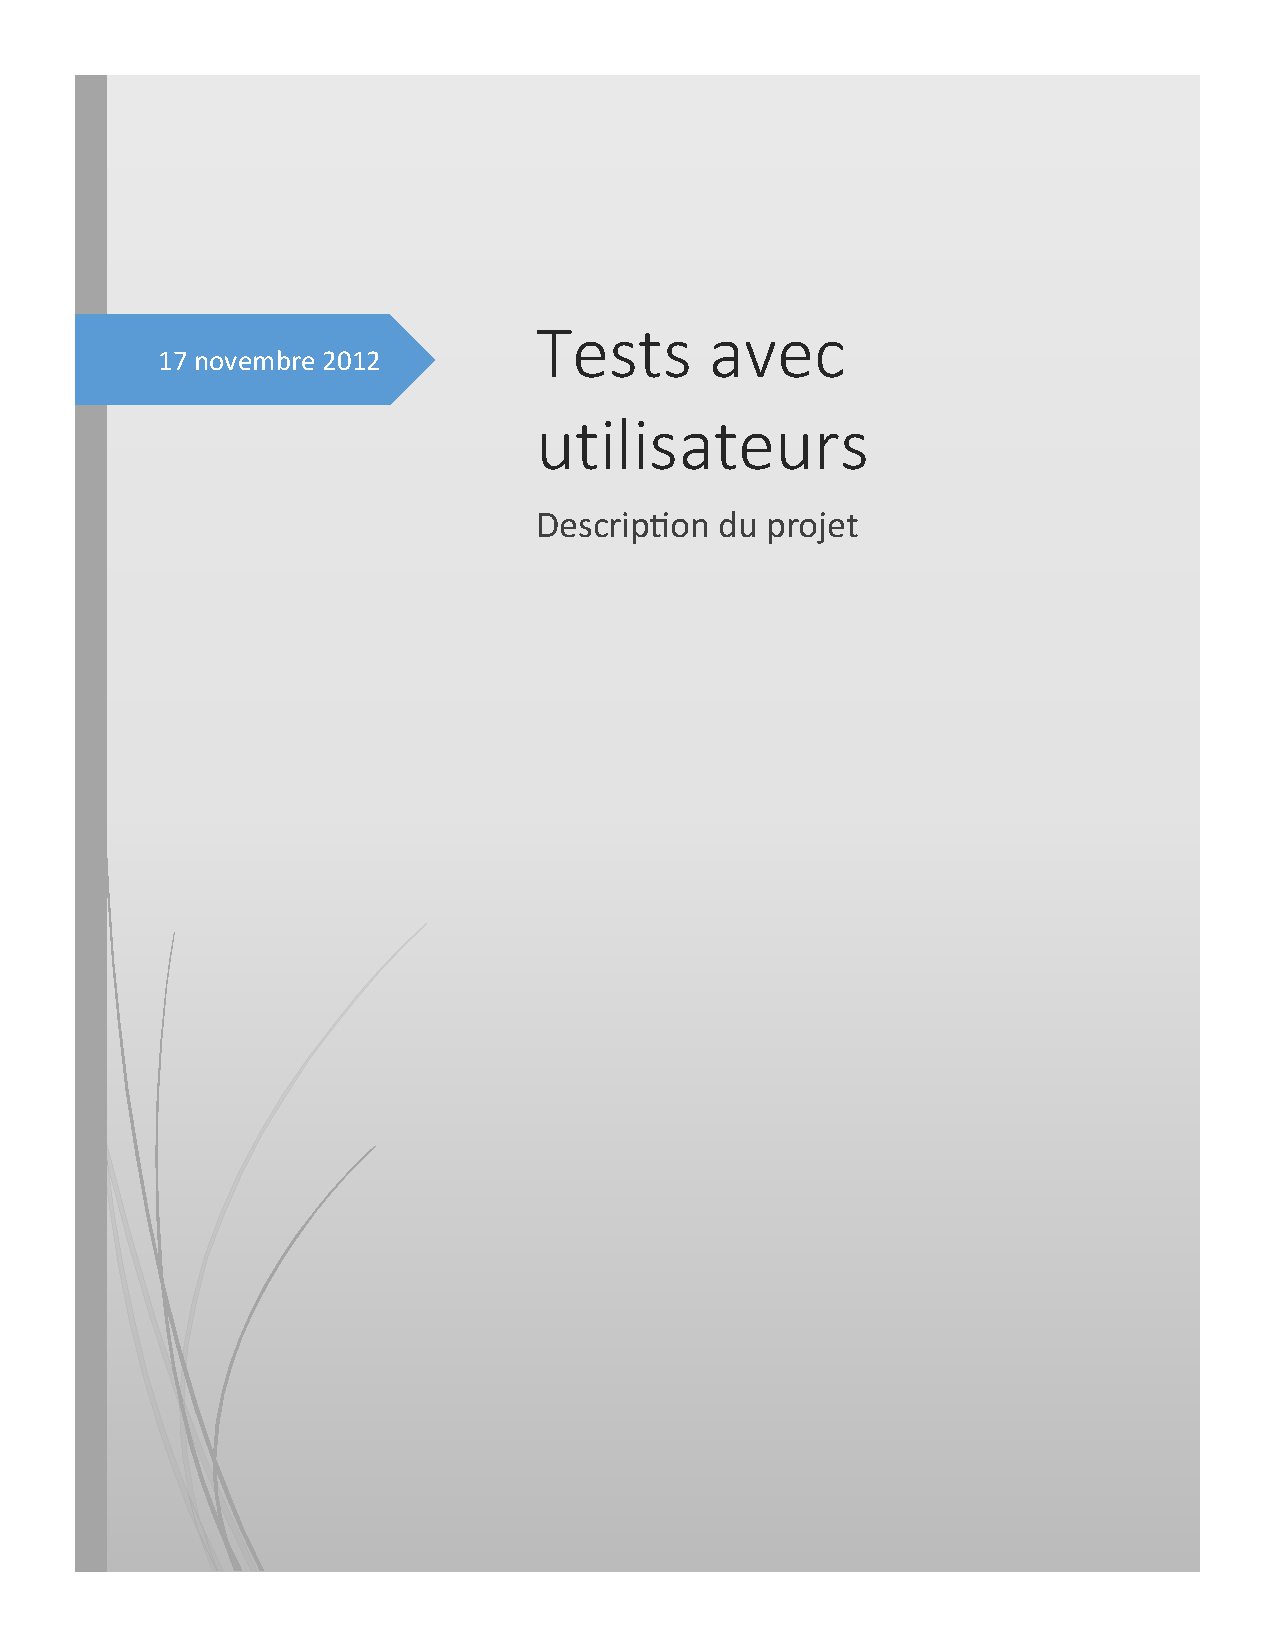
\includepdf[pages={1}]{PageTitre.pdf}

%\maketitle

\tableofcontents

\listoftables

%\listoffigures

\chapter{Contenu du document}

Le présent document contient une présentation du projet ainsi qu'une description des différentes évaluations $:$ les méthodologies, le déroulement de l'évaluation ainsi qu'un exemple des fiches qui seront utilisées durant l'évaluation.

Ce document se veut à but descriptif afin bien comprendre le contexte de l'application et le but de l'évaluation.

\chapter{Glossaire}

\begin{description}
\item [Tâche] Travail à effectuer
\item [Échéance] Date limite pour effectuer un travail
\item [Alerte] Rappel avant une date
\item [Événement] Activité, occurrence à une date donnée
\end{description}

\glsaddall
\printglossaries

\chapter{Présentation de l'application}

\section{Description de l'application}

L’application permet la gestion simple de tâches et d’événements tout en offrant des fonctionnalités de gestion et de classification avancées. Parmi celles-ci, notons la possibilité de définir des rappels, de catégoriser les éléments, de définir un événement comme échéance d'une tâche ou encore de définir des sous-tâches à une tâche imposante.

Le système de classification modulaire permet à l'utilisateur de définir des listes thématiques n'affichant que les informations pertinentes dans un contexte défini. Par exemple, l'on pourrait définir une liste « Université » n'affichant que les tâches non complétées catégorisées comme du travail universitaire ou bien une liste « Tâches urgentes » n'affichant que les tâches non complétées dont l'échéance se trouve dans prochaines 48 heures, indépendamment de leur catégorie.

Ces fonctionnalités avancées ne signifient nullement que l'application est complexe ou réservée au professionnels. L'application n'oblige jamais d'en faire plus que nécessaire. En fait, si aucune gestion avancée n'est nécessaire, une tâche peut être réduite à un strict minimum : un nom. En effet, il n'est pas très utile de définir une échéance pou la tâche « Acheter du lait et une miche de pain ».

Lors d'une utilisation quotidienne, les tâches et événements sont généralement créés de façon itérative. Par exemple, un étudiant assiste à un cours et l'enseignant lui indique qu'il devra remettre son travail de session le jour de l'examen final. Bien sûr, la date de l'examen ne sera définie que bien plus tard. Qu'à cela ne tienne, notre étudiant crée un événement « Examen du cours de ... » et l'assigne à la catégorie « Université » sans en définir de date. Il crée ensuite une tâche « Travail de session » dans la même catégorie et lui assigne le nouvel événement comme échéance. L'enseignant indique alors que le travail sera constitué de trois parties : une analyse de situation, la réalisation du projet et un rapport. Notre étudiant crée alors une sous-tâche pour chaque partie.

Notre étudiant peut maintenant garder un oeil sur son travail de session dans la liste « Université » où il regroupe tout ce qui a trait à ses études.

\section{Contexte du domaine d’application et motivation}

Dans le monde moderne, tout va toujours extrêmement vite : des rendez-vous, des conférences, des fêtes, des travaux à remettre des entretiens à faire, des pneus à changer, etc. L'homme moderne doit être à même de gérer un très grand nombre d'obligations et de choses à faire. Clairement, il doit y avoir une façon de s'y retrouver dans tout ça. La façon la plus simple est de simplement utiliser sa mémoire. Seulement, cette technique montre rapidement ses limites lorsque le nombre d'éléments dont il faut se souvenir augmente. Il devient alors nécessaire d'utiliser un outil plus fiable.

Au début une simple liste sur un bout de papier peut faire l'affaire. Vient ensuite l'utilisation d'un calendrier ou encore d'un agenda. Dans des environnements professionnels, des logiciels d'envergures sont utilisés pour soutenir la gestion des choses à faire : on peut penser à Outlook, Trac ou encore Microsoft Project.

Pour beaucoup de gens, la plupart des solutions disponibles sont soit trop simples, soit trop complexes. Le besoin de développer une solution plus puissante tout en restant simple était évident. Pour répondre à ce besoin, nous avons développé un outil léger et efficace qui permet d'offrir une gestion des tâches et événements. Avec cet outil, il est donc possible d'effectuer un suivi des choses à faire et des événements auxquels assister. Lorsqu'une unique liste devient trop volumineuse, il est possible de modifier le classement comme bon nous semble. Par exemple, il peut sembler logique de classer ses tâches par sujet, mais il peut être tout aussi logique de les classer par échéance si ce qui doit être fait d'ici un mois n'est pas pertinent dans le contexte actuel.

\section{Description du public cible et des types d’intervenants}

L'utilisateur cible est une personne cherchant à organiser son temps et sa vie professionnelle de façon simple et efficace. Cette personne doit avoir accès à un ordinateur et connaître les rudiments de base de son utilisation tels que la manipulation de fenêtre et la saisie de données.

\chapter{Description de l'évaluation}

\section{Méthodologies utilisées}

Les tests effectués seront les suivants :
\begin{description}
\item [psychomoteurs] \hfill \\ Relatif aux fonctions psychiques et motrices \footnote{\url{http://dictionnaire.reverso.net/francais-definition/psychomoteur}}
\item [de performance] \hfill \\ Test dont l'objectif est de déterminer la performance d'un système informatique \footnote{\url{https://fr.wikipedia.org/wiki/Test_de_performance}}
\item [d’usabilité (tests, enquêtes et focus groups)] \hfill \\ Consiste à observer directement l'utilisateur en train de se servir de l'application \footnote{\url{http://www.usabilis.com/methode/test-utilisateur.htm}}
\end{description}

\section{Déroulement de l'évaluation}

Chaque évaluation se déroulera en présence de l'évaluateur et celui-ci dictera les action qui devront être effectuées. Durant la réalisation du test, l'évaluateur prendra des notes ayant trait aux résultats du test, aux difficultés rencontrées ainsi que toute autre observation jugée pertinente.

De plus, l'utilisateur pourra donner son point de vue sur des améliorations possibles ou bien critiquer les défauts que celui-ci voit dans l'application.

\section{Exemple}

\subsection{Fiche de tâches à effectuer}

Cette fiche contient les tâches que l'évaluateur demandera à l'utilisateur d'effectuer.

\begin{table}[H]
\centering
\begin{tabular}{|l|l|l|}
	\hline
	No de tâche & Titre et description & Éléments que vous voulez vérifier et hypothèses \\ \hline
	1 & Ajouter une tâche en utilisant & L'utilisation des raccourcis disponible pour \\
	   & la barre d'ajout rapide. &  l'utilisateur. \\ \hline
	\dots & \dots & \dots \\ \hline
\end{tabular}
\caption{Tâches à effectuer}
\end{table}

\newpage

\subsection{Fiche de discussion et recommandation}

C'est dans cette fiche que l'évaluateur noteras les observations effectuées sur l'utilisateur et les recommandations que l'utilisateur mentionne à l'évaluateur.

\begin{table}[H]
\centering
\begin{tabular}{|l|l|l|}
	\hline
	no Tâche & Points importants de l’observation de A & Recommandations \\ \hline
	1 & L'utilisateur ne trouve pas comment & Rendre l'option plus visible et \\
	   & ajouter. & intuitive. \\ \hline
	\dots & \dots & \dots \\ \hline
\end{tabular}
\caption{Discussion et recommandation}
\end{table}

\end{document}
